\section{Implementation Details}

\subsection{Autoencoder Architecture}

The detailed architecture of the EMGSpecAutoEncoder is as follows:

\begin{table}[h]
    \centering
    \caption{EMGSpecAutoEncoder Architecture}
    \begin{tabular}{lll}
        \toprule
        Layer                    & Output Shape  & Parameters \\
        \midrule
        \multicolumn{3}{c}{Encoder}                           \\
        \midrule
        Input                    & (B, 32, T, F) & -          \\
        Conv2D (3×3, 16 filters) & (B, 16, T, F) & 4,624      \\
        BatchNorm2D              & (B, 16, T, F) & 32         \\
        ReLU                     & (B, 16, T, F) & -          \\
        \midrule
        \multicolumn{3}{c}{Decoder}                           \\
        \midrule
        Conv2D (3×3, 32 filters) & (B, 32, T, F) & 4,640      \\
        \bottomrule
    \end{tabular}
\end{table}

Where B is the batch size, T is the time dimension, and F is the frequency dimension.

\subsection{Multi-Scale TDS Convolution Block}

The detailed implementation of the MultiScaleTDSConv2dBlock is as follows:

\begin{algorithm}
    \caption{MultiScaleTDSConv2dBlock Forward Pass}
    \begin{algorithmic}[1]
        \STATE \textbf{Input:} x (input tensor), channels, width, kernel\_widths=[$k_1$, $k_2$, $k_3$]
        \STATE \textbf{Output:} y (output tensor)
        \STATE // Reshape for 2D convolutions: TNC -> NCHW
        \STATE x\_reshaped = Reshape(x) to (N, channels, width, T)
        \STATE // Apply multi-scale convolutions in parallel
        \STATE features\_1 = Conv2d(x\_reshaped, channels, kernel\_size=(1, $k_1$))
        \STATE features\_2 = Conv2d(x\_reshaped, channels, kernel\_size=(1, $k_2$))
        \STATE features\_3 = Conv2d(x\_reshaped, channels, kernel\_size=(1, $k_3$))
        \STATE // Find minimum time dimension among all features
        \STATE min\_time = Min(features\_1.shape[3], features\_2.shape[3], features\_3.shape[3])
        \STATE // Trim all features to the minimum time dimension
        \STATE features\_1 = features\_1[..., :min\_time]
        \STATE features\_2 = features\_2[..., :min\_time]
        \STATE features\_3 = features\_3[..., :min\_time]
        \STATE // Concatenate along the channel dimension
        \STATE x\_concat = Concatenate([features\_1, features\_2, features\_3], dim=1)
        \STATE // Merge features using 1×1 convolution
        \STATE x\_merged = Conv2d(x\_concat, channels, kernel\_size=1)
        \STATE x\_merged = ReLU(x\_merged)
        \STATE // Reshape back: NCHW -> TNC
        \STATE x\_out = Reshape(x\_merged) to (T\_out, N, channels * width)
        \STATE // Add residual connection
        \STATE residual = x[-T\_out:]
        \STATE y = x\_out + residual
        \STATE // Apply layer normalization
        \STATE y = LayerNorm(y)
        \STATE \textbf{return} y
    \end{algorithmic}
\end{algorithm}

\subsection{Training Hyperparameters}

The hyperparameters used for training the autoencoder and the main model are as follows:

\begin{table}[h]
    \centering
    \caption{Training Hyperparameters}
    \begin{tabular}{lll}
        \toprule
        Hyperparameter          & Autoencoder & Main Model      \\
        \midrule
        Optimizer               & Adam        & Adam            \\
        Learning rate           & 1e-3        & 1e-3            \\
        Batch size              & 32          & 32              \\
        Training epochs         & 150         & 150             \\
        Early stopping patience & 10          & 10              \\
        Learning rate scheduler & None        & CosineAnnealing \\
        \bottomrule
    \end{tabular}
\end{table}

\section{Additional Results}

\subsection{Learning Curves}

\subsubsection{Autoencoder}
\begin{figure}[h]
    \centering
    \begin{minipage}{0.48\textwidth}
        \centering
        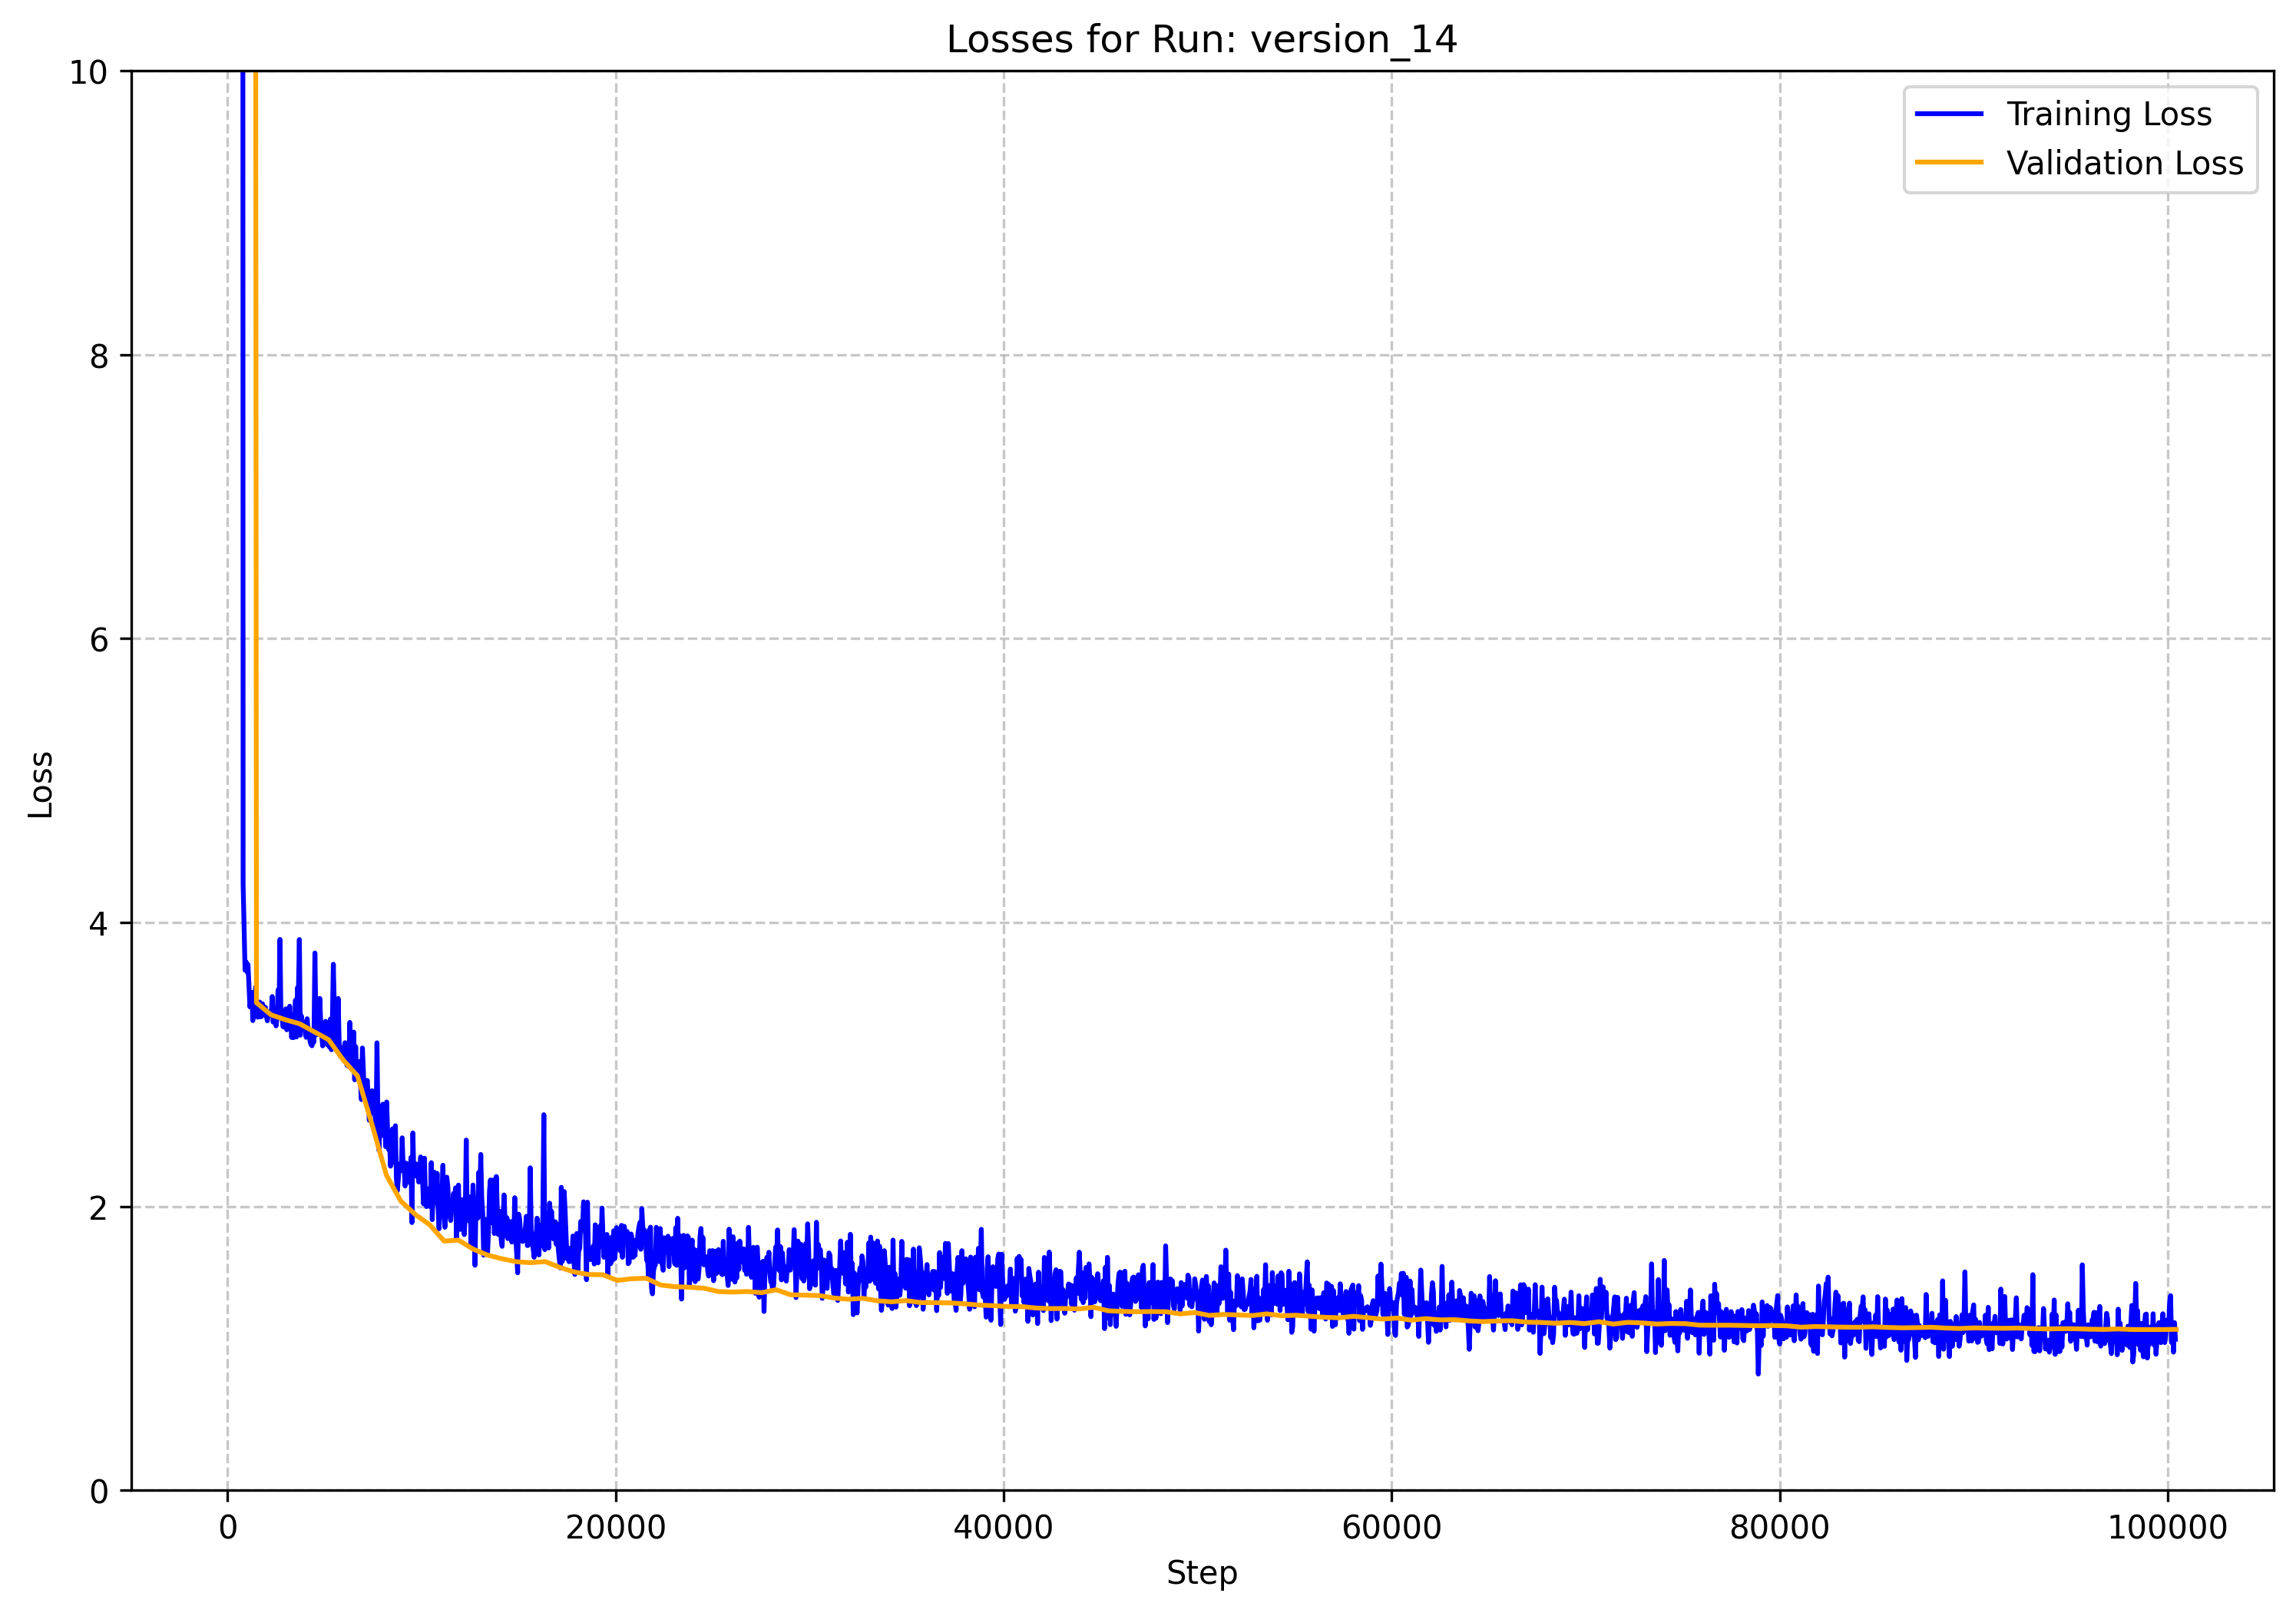
\includegraphics[height=7cm,width=\textwidth]{../results/model-autoencoder-tiny/model-autoencoder-tiny_losses.png}
        \caption{Learning curves showing training and validation loss for the autoencoder}
        \label{fig:autoencoder_loss}
    \end{minipage}
    \hfill
    \begin{minipage}{0.48\textwidth}
        \centering
        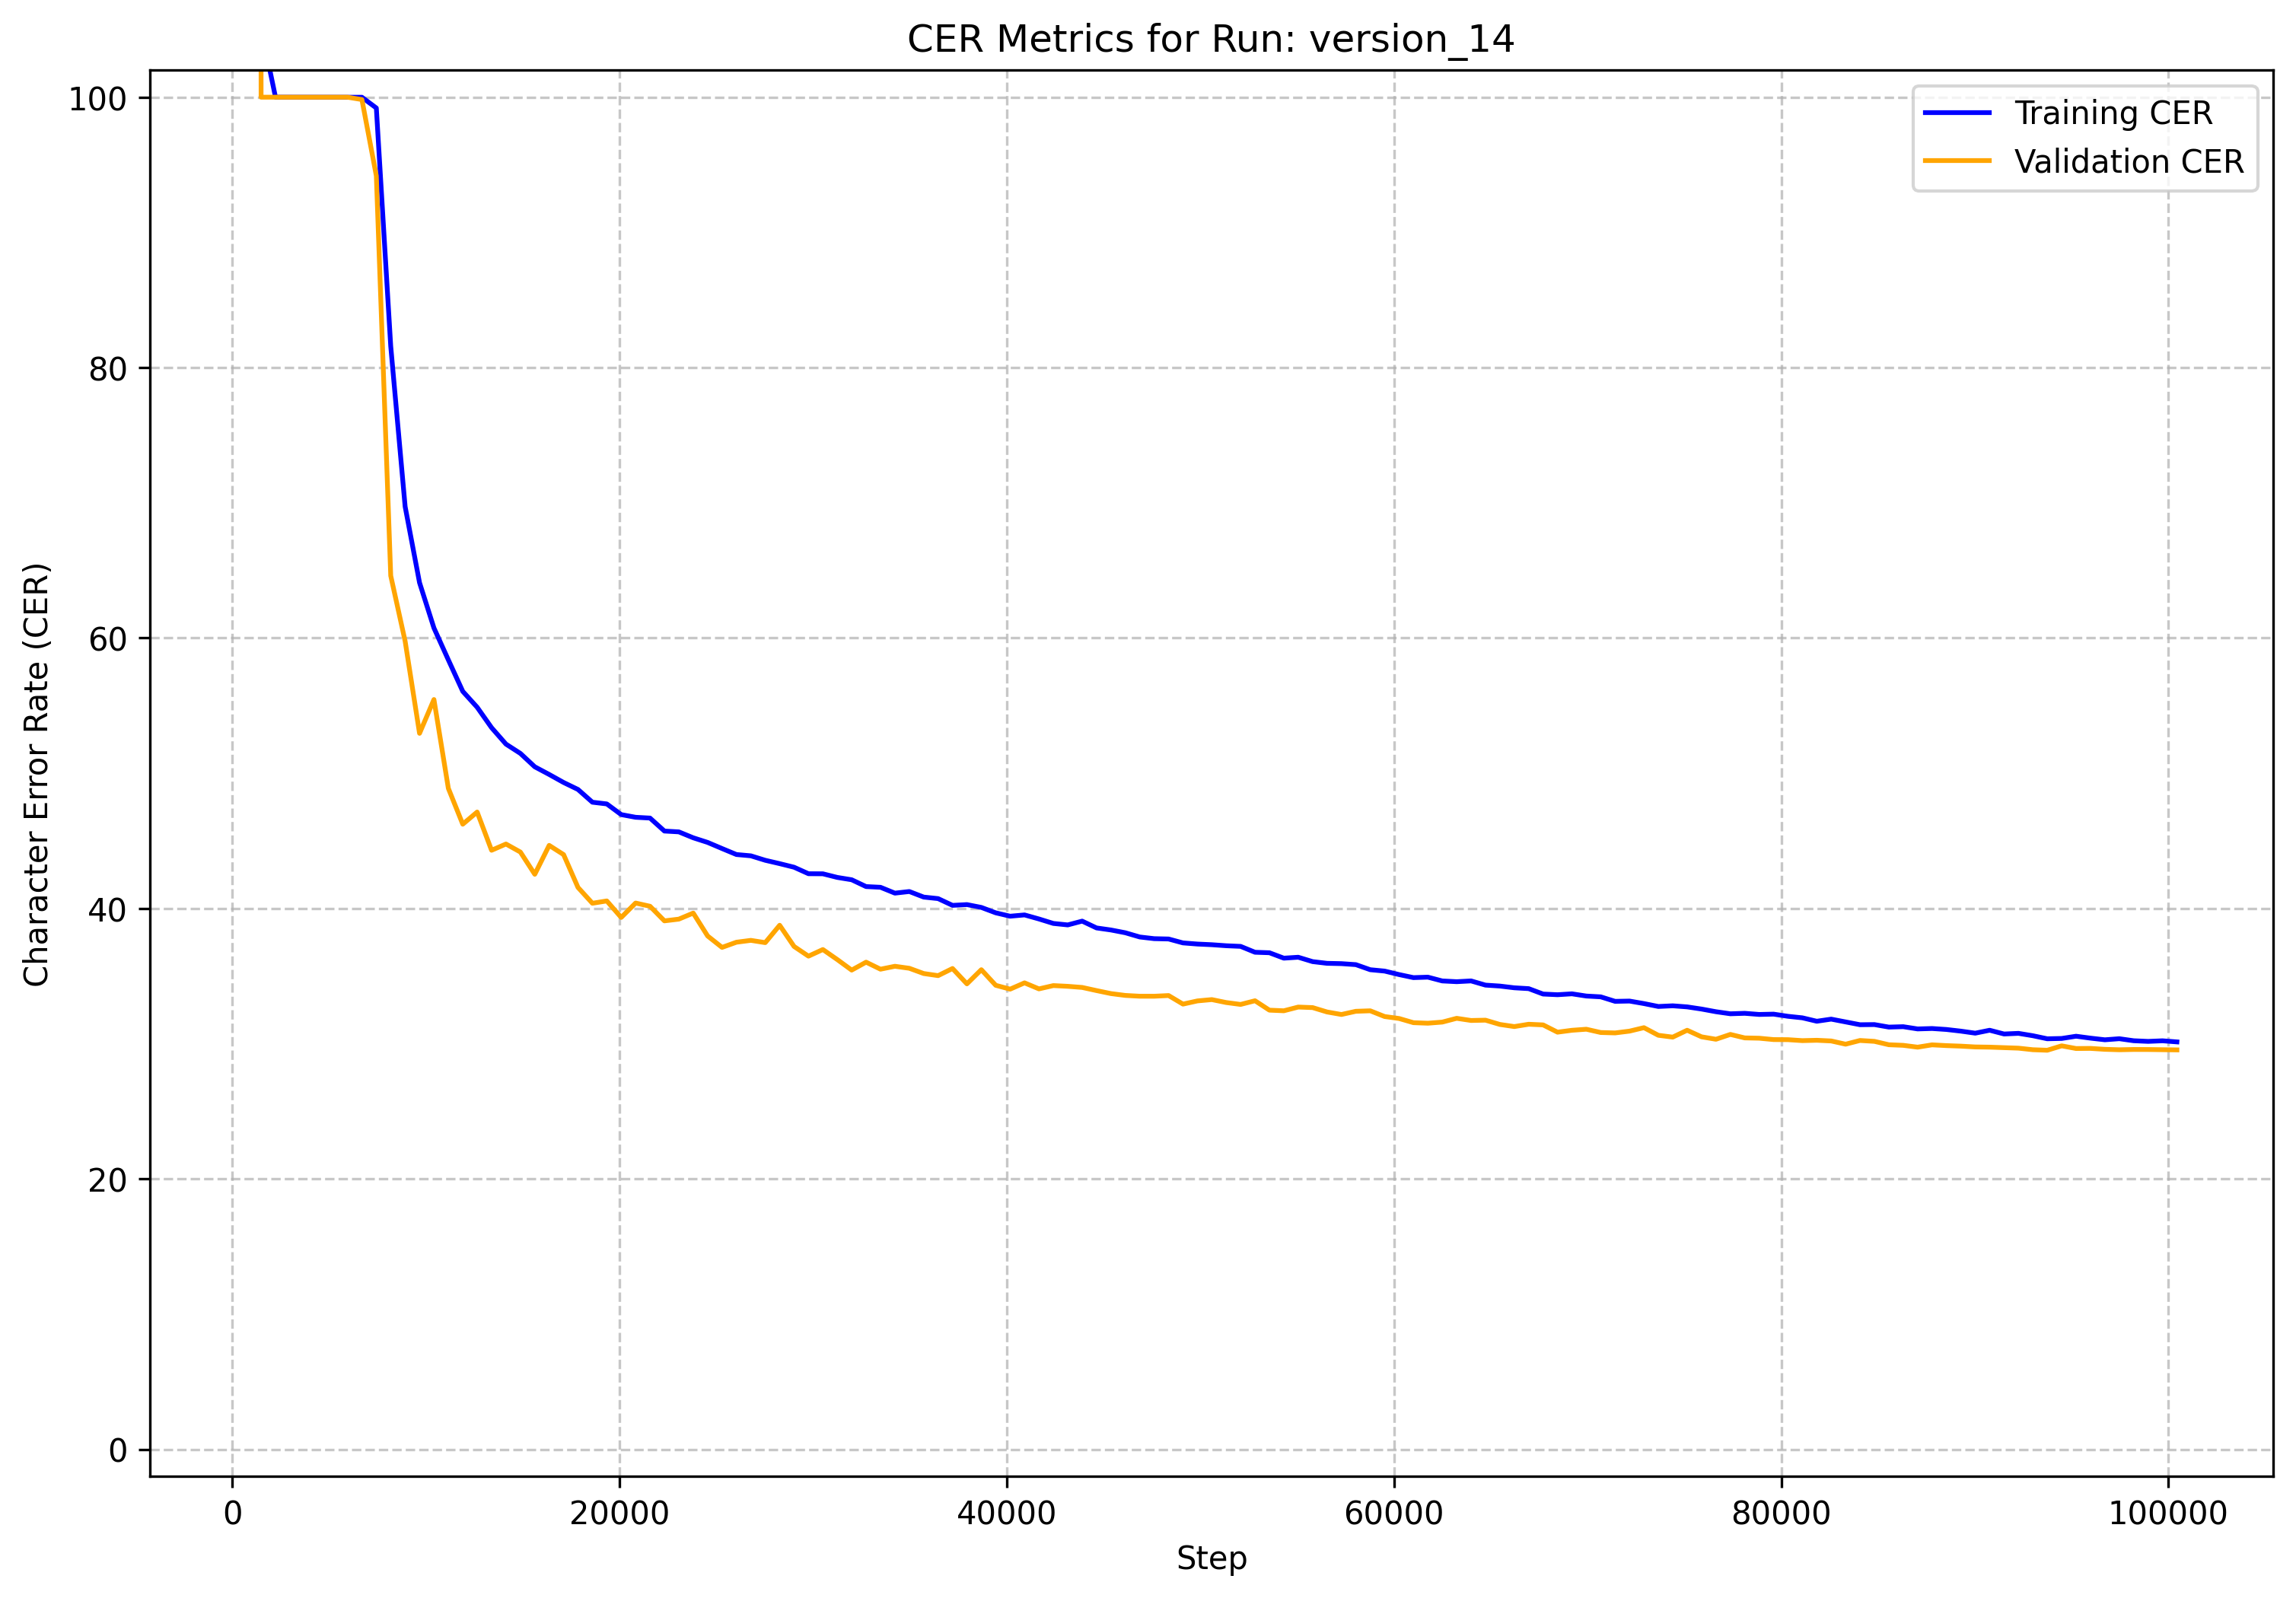
\includegraphics[height=7cm, width=0.8\textwidth]{../results/model-autoencoder-tiny/model-autoencoder-tiny_cer.png}
        \caption{Learning curves showing training and validation CER for the autoencoder}
        \label{fig:autoencoder_cer}
    \end{minipage}
\end{figure}

\subsubsection{Multi-Scale TDS Convolution Model}
\begin{figure}[h]
    \centering
    \begin{minipage}{0.48\textwidth}
        \centering
        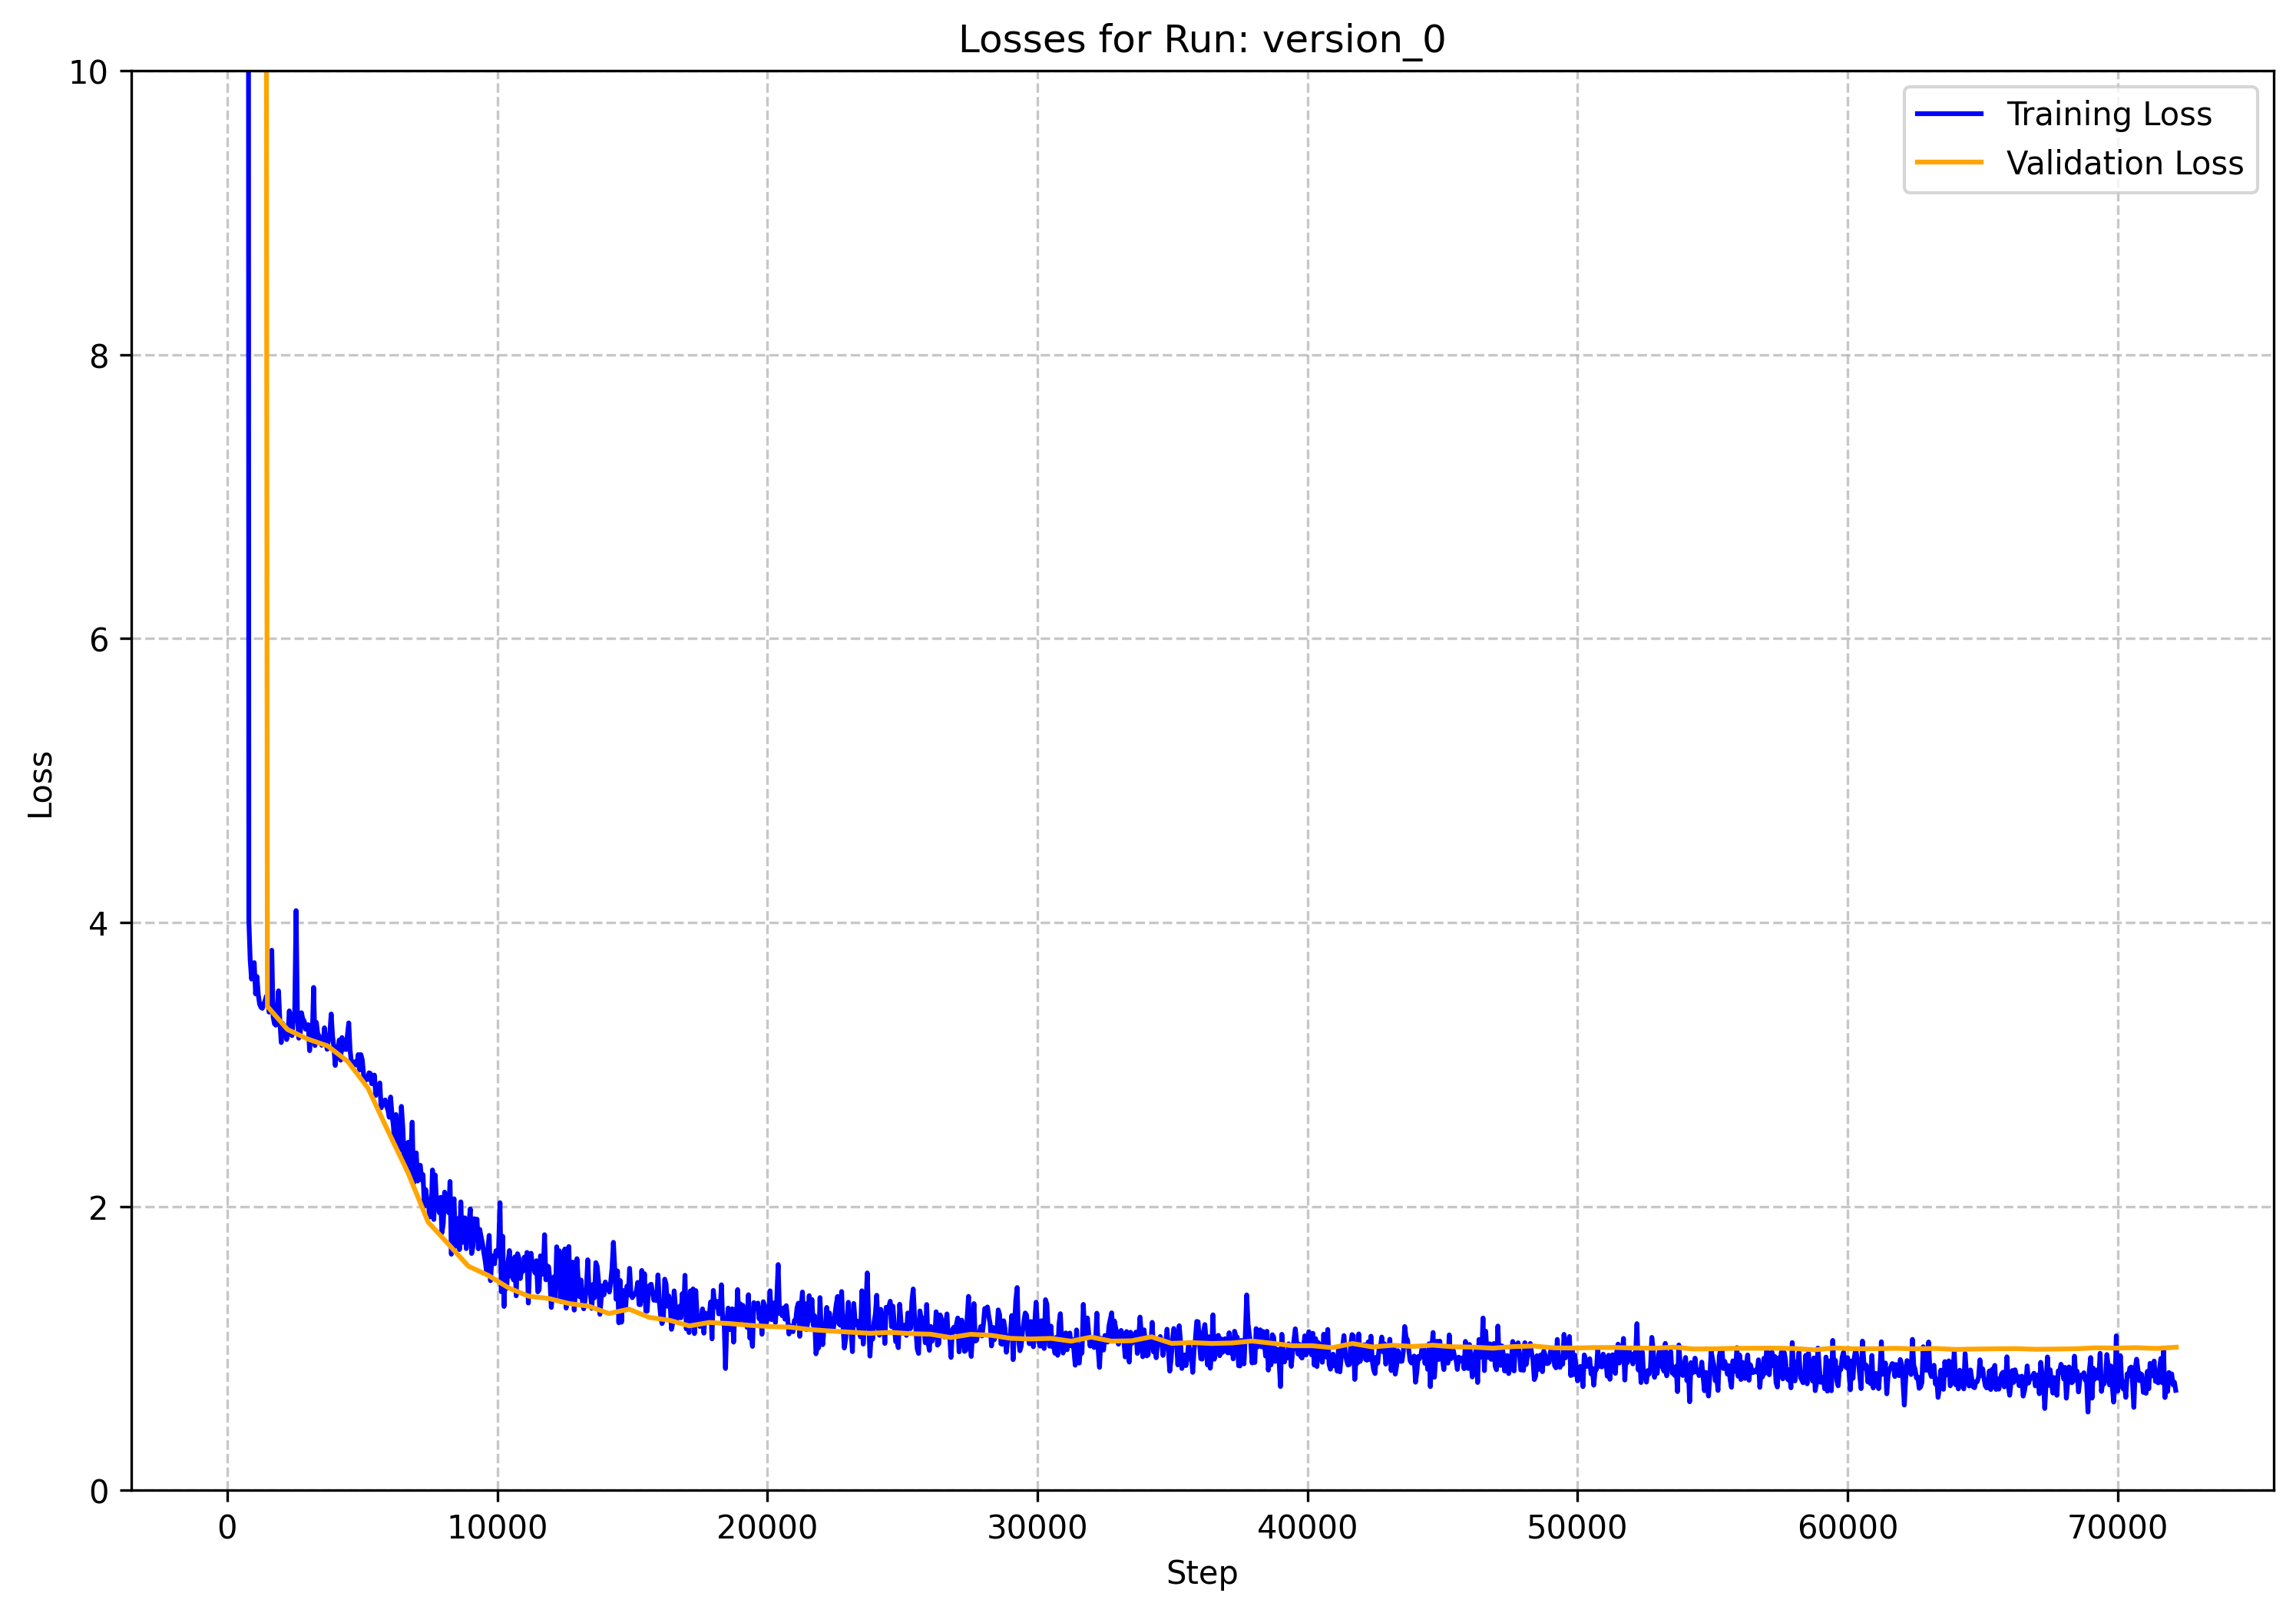
\includegraphics[height=7cm,width=\textwidth]{../results/model-multi-scale-tiny/model-multi-scale-tiny_loss.png}
        \caption{Learning curves showing training and validation loss for the multi-scale TDS convolution model}
        \label{fig:multi_scale_loss}
    \end{minipage}
    \hfill
    \begin{minipage}{0.48\textwidth}
        \centering
        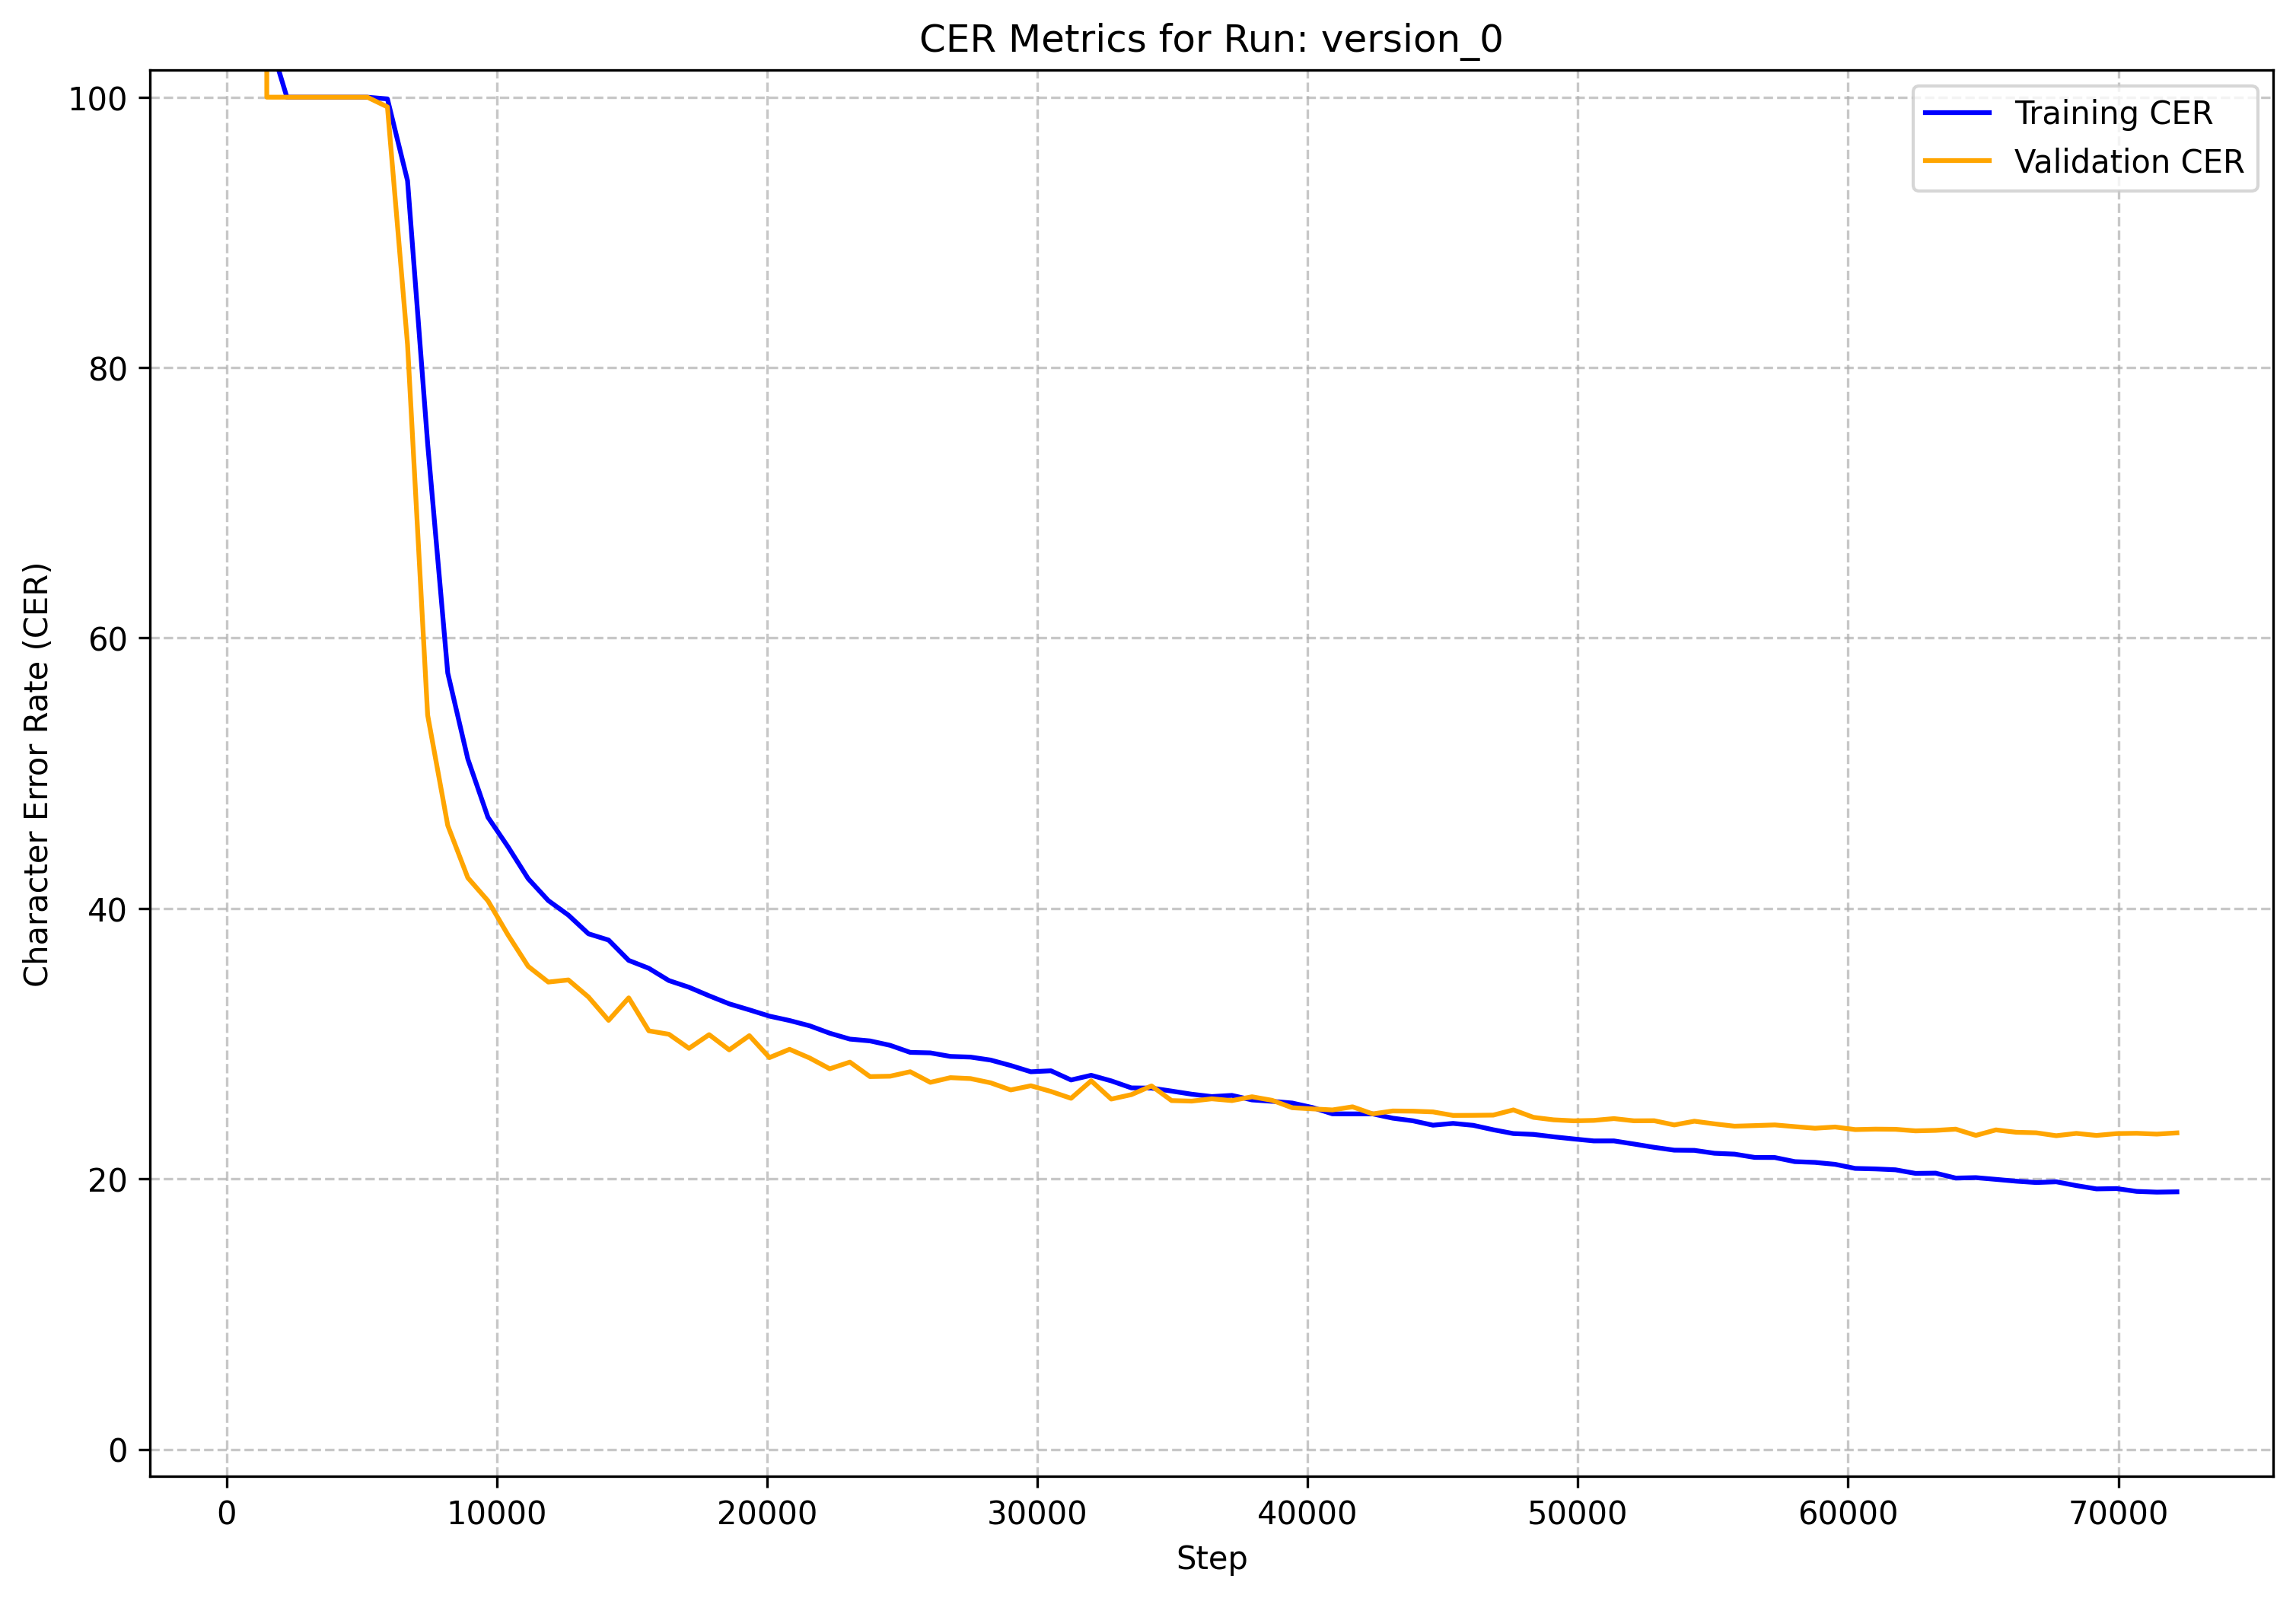
\includegraphics[height=7cm, width=0.8\textwidth]{../results/model-multi-scale-tiny/model-multi-scale-tiny_cer.png}
        \caption{Learning curves showing training and validation CER for the multi-scale TDS convolution model}
        \label{fig:multi_scale_cer}
    \end{minipage}
\end{figure}

\subsubsection{Autoencoder and Multi-Scale TDS Convolution Model}
\begin{figure}[h]
    \centering
    \begin{minipage}{0.48\textwidth}
        \centering
        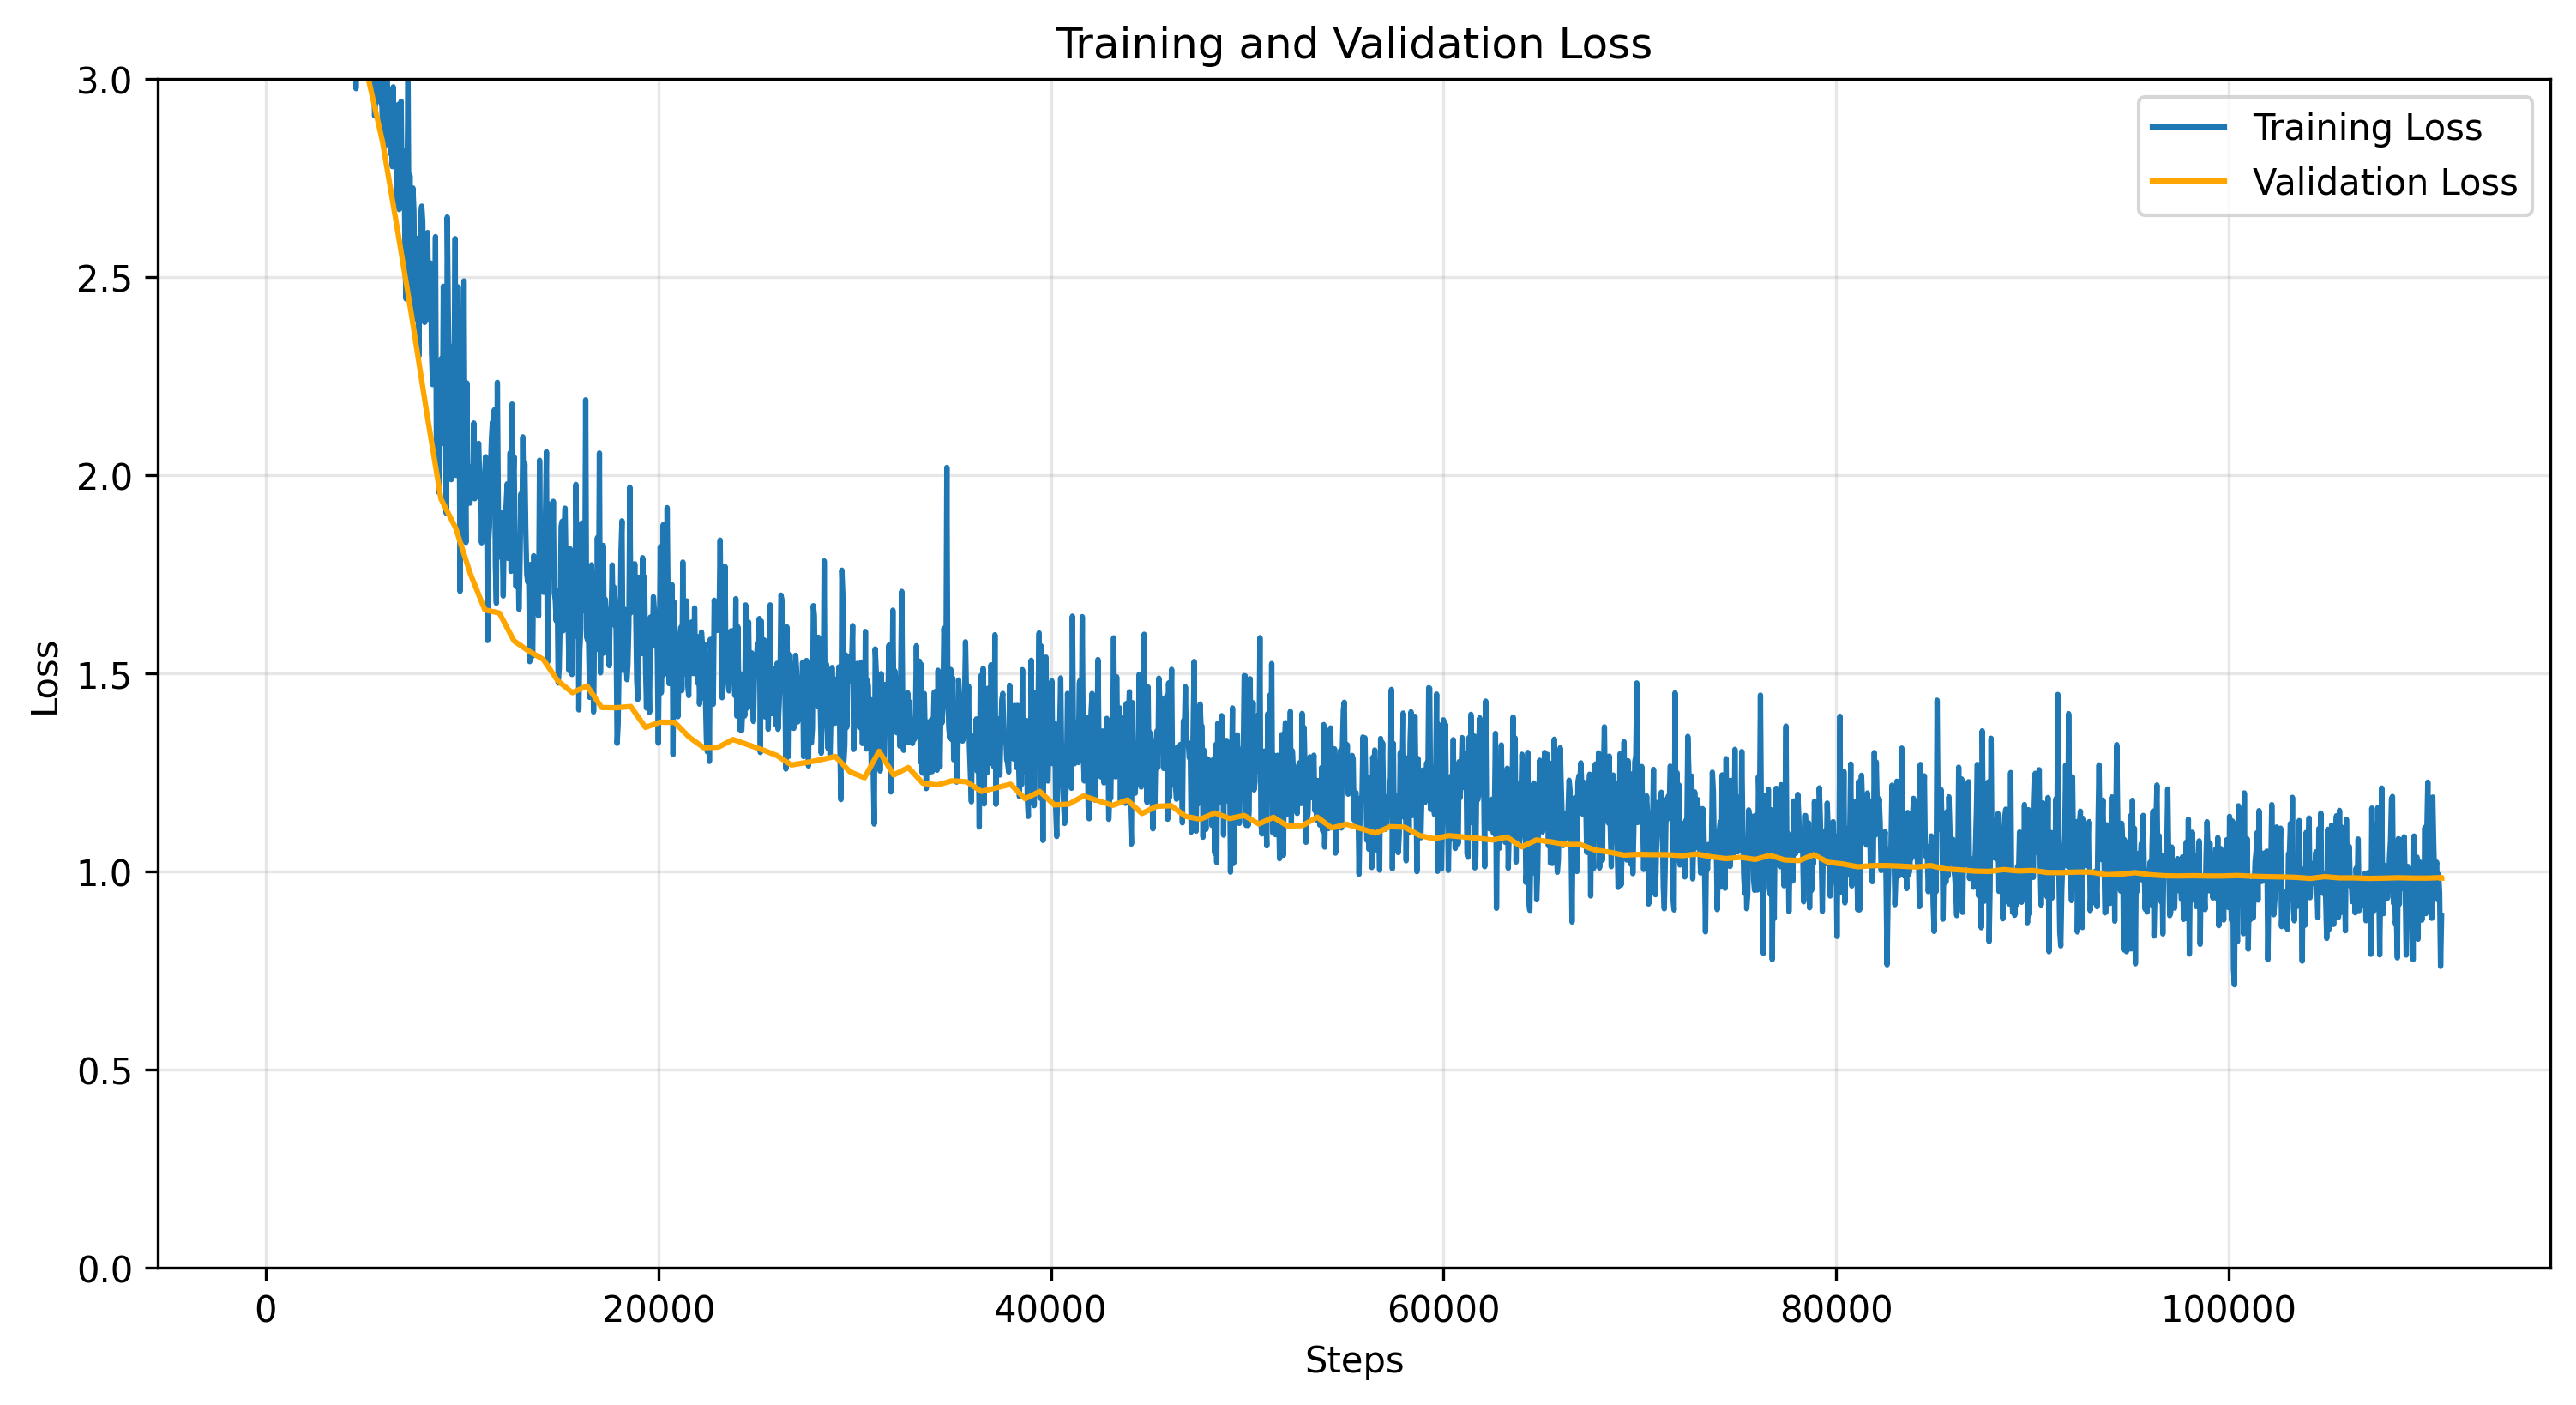
\includegraphics[height=7cm,width=\textwidth]{../results/model-multi-scale-autoencoder-tiny/loss_plot.png}
        \caption{Learning curves showing training and validation loss for the autoencoder and multi-scale TDS convolution block}
        \label{fig:autoencoder_multi_scale_loss}
    \end{minipage}
    \hfill
    \begin{minipage}{0.48\textwidth}
        \centering
        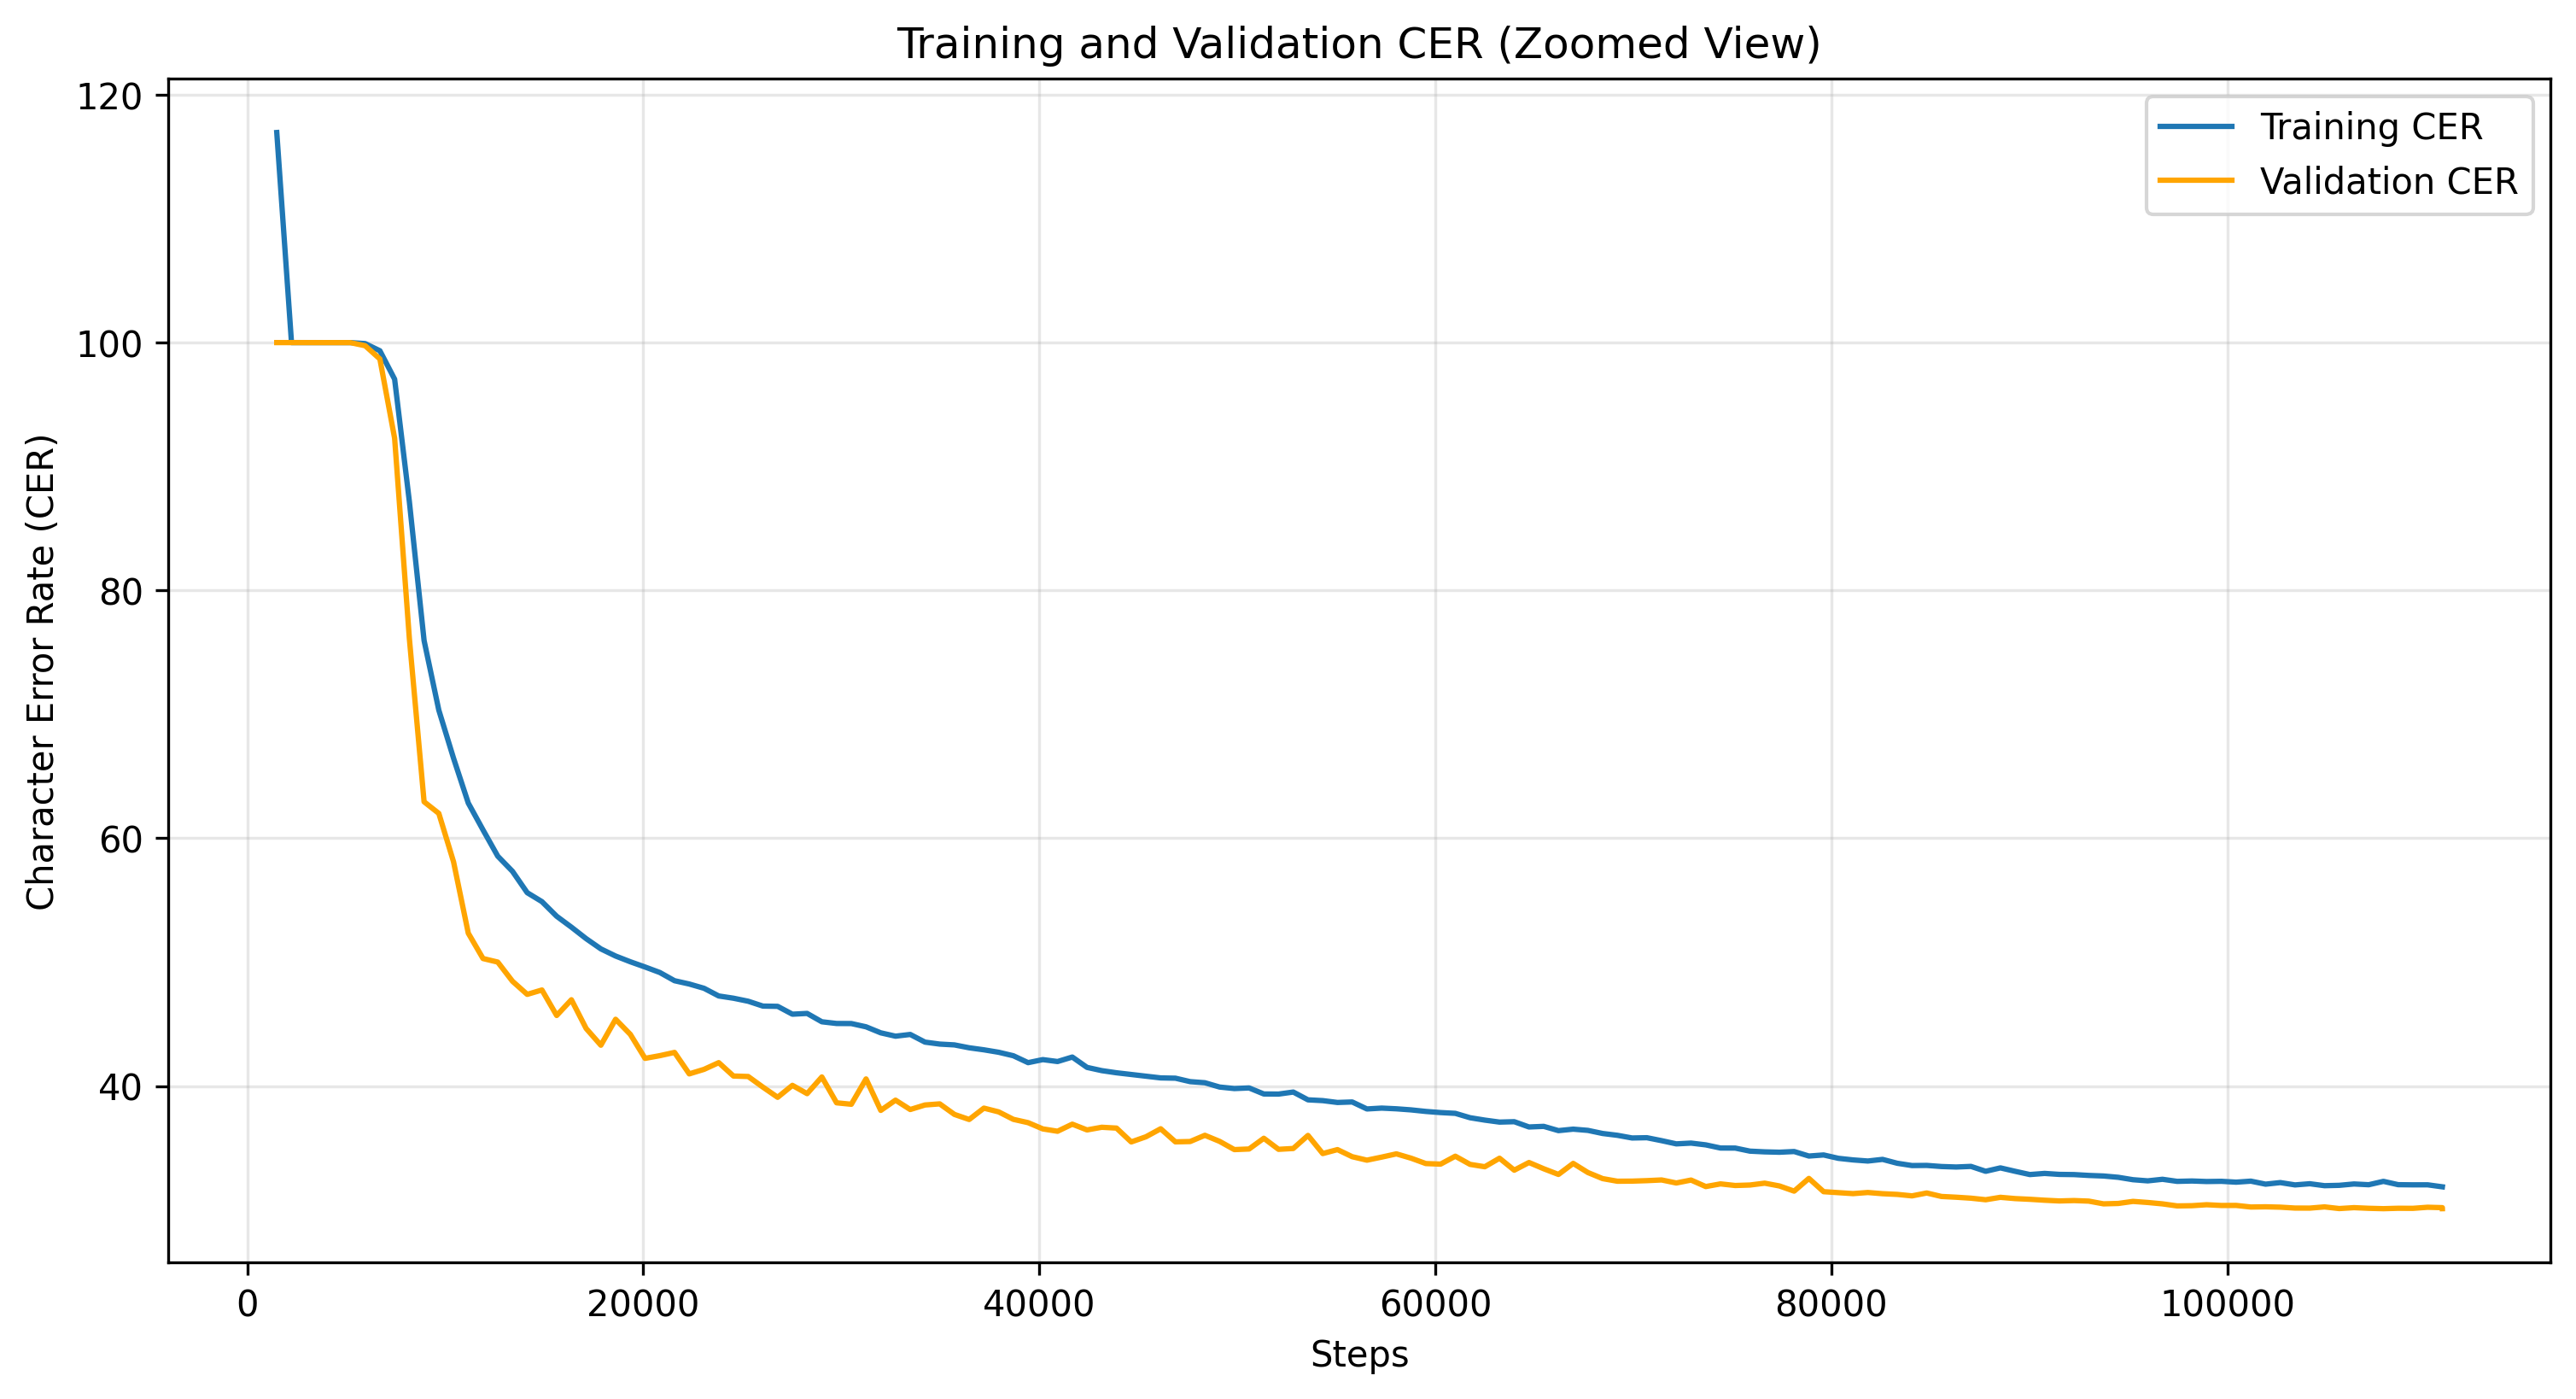
\includegraphics[height=7cm, width=0.8\textwidth]{../results/model-multi-scale-autoencoder-tiny/cer_zoomed_plot.png}
        \caption{Learning curves showing training and validation CER for the autoencoder and multi-scale TDS convolution block}
        \label{fig:autoencoder_multi_scale_cer}
    \end{minipage}
\end{figure}

\subsection{Feature Visualization}

[FIGURE: t-SNE visualization of the bottleneck features colored by character]

\subsection{Error Analysis}

[TABLE: Most common character confusions]

[FIGURE: Confusion matrix for character prediction]

\subsection{User-Specific Performance}

[TABLE: CER breakdown by user]

[FIGURE: Bar chart comparing baseline and proposed model performance across users]